\documentclass[11pt,a4paper,twoside]{article}

% You should not change the line above.
% Nor change any of the formating.

% At a minimum, you need to edit the preamble file for your name and project
% title. There are a lot of latex commands there you might find useful.
\usepackage[a4paper]{geometry}
\usepackage{amsfonts}
\usepackage{amsthm}
\usepackage{amsmath}
\usepackage{parskip}
\usepackage{mathrsfs}
\usepackage{graphicx}
\usepackage{amssymb}
\usepackage{xtab}

% You need to set the next two items. 
% If you title is long, you may need to adjust the spacing in titlepage.tex
\newcommand{\TheAuthor}{Your Name}
\newcommand{\TheTitle}{Your Project title}

% uncomment exacly one of these
\newcommand{\TheModule}{\bf MA4K8 Scholarly Report}
%\newcommand{\TheModule}{\bf MA4K9 Dissertation}


% Leave the following two as is
\newcommand{\TheUni}{The University of Warwick}
\newcommand{\TheDept}{Mathematics Institute}

% Set the correct submission year, e.g. replace 2000 with 2017
\newcommand{\TheSubDate}{\monthyear \formatdate{5}{4}{2000}}

% The are a lot of things you might find useful and want to uncomment. 
% Most things you will want to uncomment or change will be near the top.

% standard maths symbols (you probably want to uncomment all of these)
% \newcommand{\Z}{\ensuremath{\mathbb{Z}}}% integers
% \newcommand{\N}{\ensuremath{\mathbb{N}}}% natural numbers
% \newcommand{\R}{\ensuremath{\mathbb{R}}}% real numbers
% \newcommand{\C}{\ensuremath{\mathbb{C}}}% complex numbers

% Others 
%\newcommand{\st}{\ensuremath{:}}% such that
%\newcommand{\Tau}{\ensuremath{\mathcal{T}}}
%\newcommand{\Nat}{\mathbb{N}}

%\usepackage[numbers]{natbib}% round braces, sort multiple citations
%\usepackage{hyperref}% creates hypertext links in pdf files (natbib compatible)
\usepackage{setspace}
%\usepackage{fancyhdr}
%\usepackage{mathrsfs}
%\usepackage{textcomp}
%\usepackage{color}
%\usepackage{graphicx}
%\usepackage{framed}
% \usepackage{algorithmic}% format pseudocode
%\usepackage[vlined,boxed,commentsnumbered,algochapter]{algorithm2e}
% \usepackage[chapter]{algorithm}% float wrapper for algorithms
%\usepackage{amsmath}% American Mathematical Society macros - essential!
%\usepackage{amssymb}% contains amsfonts
%\usepackage{amsthm}% allows more flexibility with theorems
\usepackage[nodayofweek]{datetime} % change the format of printed dates (no american style!) 
%\usepackage{ifdraft}% perform operations conditional on the draft option

% \usepackage{mathptmx}
% \usepackage{mathpazo}
%\usepackage{amscd}
% \usepackage{xy}
% \usepackage{diagxy}
%\usepackage{diagrams}

%\usepackage{marginnote}
%\usepackage{rotating}
%\usepackage{multirow}
% \usepackage{polski}
% \usepackage[T1]{fontenc}
% \usepackage{tikzpicture}
% \usetikzlibrary{matrix,arrows}

% \usepackage[inline]{showlabels}
%\usepackage{booktabs}

% Date format

% Use the datetime package
\newdateformat{monthyear}{\monthname[\THEMONTH], \THEYEAR}% new date format

% New commands, operators and symbols

% Operators
%\DeclareMathOperator{\Sym}{Sym}% symmetric group
%\DeclareMathOperator{\Alt}{Alt}% alternating group
%\DeclareMathOperator{\Id}{Id}
%\DeclareMathOperator{\Hom}{Hom}
%\DeclareMathOperator{\Grp}{Grp}
%\DeclareMathOperator{\supp}{supp}
%\DeclareMathOperator{\fix}{fix}
%\DeclareMathOperator{\dep}{dep}
%\DeclareMathOperator{\lcm}{lcm}
%\DeclareMathOperator{\Aut}{Aut}
%\DeclareMathOperator{\Inn}{Inn}
%\DeclareMathOperator{\Out}{Out}
% \DeclareMathOperator{\dim}{dim}
%\DeclareMathOperator{\Syl}{Syl}
%\DeclareMathOperator{\Hall}{Hall}
%\DeclareMathOperator{\pCore}{pCore}
%\DeclareMathOperator{\Char}{char}
%\DeclareMathOperator{\Image}{Im}
%\DeclareMathOperator{\Ker}{Ker}
%\DeclareMathOperator{\Hcf}{hcf}
%\DeclareMathOperator{\GL}{GL}
%\DeclareMathOperator{\Pc}{Pc}
%\DeclareMathOperator{\Stab}{Stab}
%\DeclareMathOperator{\Orbit}{Orbit}


% Hyphenation fixes
%\newcommand{\letdash}[1]{$#1$\nobreakdash-\hspace{0pt}}% for n-element, k-transitive etc
%\newcommand{\numdash}{\nobreakdash--}

% Sequences
%\newcommand{\seqfin}[3]{\ensuremath{#1_{#2}, \dotsc , #1_{#3}}}
%\newcommand{\seqinf}[3]{\ensuremath{#1_{#2}, #1_{#3}, \dotsc}}

% New environments

% Dedication
%\newenvironment{dedication}
%{\clearpage \thispagestyle{empty} \vspace*{\stretch{1}} \begin{center} \em}
%{\end{center} \vspace*{\stretch{3}} \clearpage}


% Page Layout

% Dimensions
% Use the geometry package to set this up
\geometry{includehead,includefoot,left=3cm,right=3cm,top=2cm,bottom=2cm}% head and foot are included in total body so that nothing is printed out of the boundaries of the set margins

% Header and footer
% Use the fancydr package
%\ifdraft{%
%\fancypagestyle{plain}{% redefine plain pagestyle for draft
%\renewcommand{\headrulewidth}{0pt}% no head rule in draft mode
%\fancyhf{}% clear headers and footers
%\fancyhead[C]{\ifdraft{DRAFT}{}}% print DRAFT across top if the draft option is set
%\fancyfoot[C]{\thepage}% usual page numbering
%

%\pagestyle{fancy}
%\renewcommand{\chaptermark}[1]{\markboth{\thechapter.\ #1}{}}% compact with no capitalisation
%\renewcommand{\sectionmark}[1]{\markright{\thesection.\ #1}}% compact with no capitalisation
%\ifdraft{\renewcommand{\headrulewidth}{0pt}}{}% no head rule in draft mode
%\setlength{\headheight}{15pt}
%\fancyhf{}% clear all header and footer fields
% one-sided printing, so no E,O distinction need be made
%\fancyhead[C]{\ifdraft{DRAFT}{}}% print DRAFT across top if the draft option is set
%\fancyhead[R]{\thepage}% page in top right
%\fancyhead[L]{\ifdraft{}{\leftmark}}% chapter number and title in top left

% Theorems
%
%\newtheorem{prop}{Proposition}[chapter]
%\newtheorem{lemma}[prop]{Lemma}
%\newtheorem{conjecture}[prop]{Conjecture}
%\newtheorem{theorem}[prop]{Theorem}
%\newtheorem{hyp}[prop]{Hypothesis}
%\newtheorem{cor}[prop]{Corollary}
%\newtheorem{claim}[prop]{Claim}
%\newtheorem{remark}[prop]{Remark}
%\newtheorem{notation}[prop]{Notation}
%\newtheorem{defn}[prop]{Definition}


% Numbering
%\numberwithin{equation}{chapter}% standard style numbering, nothing special here


% Algorithms

% Use the algorithms package.
% \renewcommand{\algorithmicrequire}{\textbf{Input:}}
% \renewcommand{\algorithmicensure}{\textbf{Output:}}
% \renewcommand{\algorithmiccomment}[1]{/* #1 */}
%\RestyleAlgo{boxruled}
%\SetAlgoInsideSkip{medskip}
%\setlength{\algomargin}{2em}
%\setlength{\interspacetitleboxruled}{0.7em}
%\setlength{\interspacetitleruled}{0.7em}
%\LinesNumbered
%\SetAlCapNameSty{sc}
%\SetFuncSty{sc}

%\newenvironment{spacedalgorithm}{\begin{algorithm}\onehalfspacing}{\end{algorithm}}
% \newenvironment{onehalfverbatim}{\onehalfspacing\begin{verbatim}}{\end{verbatim}}

%\reversemarginpar
%\newcounter{nootje}
%\setcounter{nootje}{1}
%\renewcommand\check[1]{[*\thenootje]\marginnote{\tiny\begin{minipage}{40mm}\begin{flushright}\thenootje
%: #1\end{flushright}\end{minipage}}\addtocounter{nootje}{1}}


% Document details



\begin{document}

\pagenumbering{roman}
\begin{titlepage}
\begin{center}

\includegraphics[width=5cm]{Warwick_Crest} 
% this graphic file should live in the working directory
% the size of the following arguments to vspace were determined by 
% trial and error, and produce suitable output for the A4 pagesize.

\vspace*{20pt}
\begin{spacing}{2}
\begin{center}
{\Large \bf \TheTitle} % declared in preamble.tex

\vspace*{14pt}

by

{\Large \bf \TheAuthor} % declared in preamble.tex

\vspace*{16pt}

{\large \bf \TheModule} % declared in preamble.tex


Submitted to \TheUni % declared in preamble.tex

\vspace*{36pt}
{\Large \bf \TheDept} % declared in preamble.tex

\TheSubDate % declared in preamble.tex

\vspace*{36pt}

\includegraphics[width=5cm]{warwick_logo} 
% this graphic file should live in the working directory

\end{center}
\end{spacing}
\end{center}
\end{titlepage}

\setcounter{page}{2}
%\renewcommand{\contentsname}{Table of contents}
\tableofcontents
\cleardoublepage
\onehalfspacing
\pagenumbering{arabic}
\onehalfspacing
\raggedbottom

% Now starts the main part of the report. 
% Each section/chapter is in a separate file. Two examples are include.
% 
% This part (between TOC and Bibliograpy) must obey:
% for MA4K8 must not exceed 30 pages.
% for MA4K9 the target is approx 30 pages and must not exceed 40 pages.

\section{Introduction}

Consider a PDE of the following form:

\begin{align*}
    \partial_t u = N(u)\\
\end{align*}

These PDEs of this from are common when looking into Phase boundary problems such as the Allen-Cahn equations. %maybe add a citation
While for some instances exact soltions to these PDEs exist and are known, in many practical cases however it is often neccessary to compute approximate solutions to these PDEs.
In order to achieve this, we will need to discretise in space yielding an ODE.
We do this via finite element methods giving:
\begin{align*}
    M\frac d{dt} u_h = N_h(u)\\
\end{align*}
For a mass matrix $M$ and some $N_h$.
From here we can apply methods that can solve this ODE in time.


\section{Solution Schemes} \label{section:methods}
Now, we outline the methods by which the ODEs arising from the discretization of PDEs in space can be solved. 
Consider the following PDE:
\begin{align*}
    \dot u_t &= N(u)
\end{align*}
Discretizing in space gives the following:
\begin{align*}
M\dot u_h(t) &= N_h(u_h(t))\\ %\text{ where $M$ is the mass matrix}
\text{using } R(u_h(t)) &= N_h(u_h(t)) - DN(u_h(t))u_h(t) \text{ to denote the non-linear term gives}\\
M\dot u_h(t) &= DN(u_h(t))u_h(t) + R(u_h(t))\\
\dot u_h(t) &= M^{-1}(DN(u_h(t))u_h(t) + R(u_h(t)))
\end{align*}
\subsection{Methods}
We present both conventional ODE solvers such as the forwards and backwards Euler method before moving on to the exponential integrator methods.
For a time step $\tau$ we compute $u_h(t+\tau)$ in the following ways: 

\subsubsection{Forwards Euler}
The forwards Euler method is given by:
\begin{align*}
u_h(t+\tau) = u_h(t) + \tau M^{-1}N_h(u_h(t))
\end{align*}

\subsubsection{Backwards Euler}
The backwards Euler method is given by:
\begin{align*}
u_h(t+\tau) = u_h(t) + \tau M^{-1}N_h(u_h(t+\tau))
\end{align*}
As this method is implicit, we will need to employ a Newton solver.

\subsubsection{Explicit Exponential Scheme} %check this is correct%
For the explicit exponential integrator schemes we use the following formula:
\begin{align*}
u_h(t+\tau) &= e^{\tau M^{-1} DN(u_h(t))}(u_h(t) + M^{-1}R(u_h(t)))
\end{align*}


\subsubsection{First Order Exponential Integrator}
Here, we also present another integrator from Huang Et al \cite{Huang2022}
\begin{align*}
u_h(t+\tau) &= e^{\tau M^{-1} DN(u_h(t))}u_h(t) + \tau \varphi_1(\tau M^{-1} DN(u_h(t)))R(u_h(t))
\end{align*}
Where:
\begin{align*}
    \varphi_k(z) &= \int^1_0e^{(1-\theta)z}\frac{\theta^{k-1}}{(k-1)!}d\theta, k \geq 1
\end{align*}

\subsubsection{Second Order Exponential Integrator}
We also look at a second order exponential integrator \cite{Huang2022}.
\begin{align*}
    \text{writing } A &= \tau M^{-1} DN(u_h(t)) \text{ for the sake of brevity}\\
    u_h(t+\tau) &= e^{A}u_h(t) + \tau((\varphi_1(A)) - \frac 1{c}\varphi_2(A))R(u_h(t))\\
    & + \frac1{c}\varphi_2(A)R(e^{cA}u_h(t) + c\tau\varphi_1(c A)R(u_h(t)))
\end{align*}
where $c \in (0,1]$.

\subsection{Mass Matrix}
When using these schemes it is necessary to be able to compute the inverse mass matrix $M^{-1}$.
Attempting to compute the exact inverse can be computationally intensive. While for a fixed spacial discretization this may be acceptable, as it will only need to be computed once, for an adaptive grid this may be impractical.
As a result, we employ mass lumping where each row is summed up and placed on the diagonal of the matrix.
From here, computing the inverse is straightforward.

\section{Krylov Methods}
When using the above exponential integrators, we need to be able to compute the matrix exponential $e^{A}$ or, more precisely, the action of the exponential of a matrix to a vector $e^{A}v$.
For a lower dimension, computing $e^{A}v$ is computationally cheap.
However, when the dimension of the matrix $A$ is large, then computing $e^{A}v$ is computationally intensive.
One solution to this is to use Krylov subspace methods.
These algorithms take a matrix $A\in \mathbb{R}^{n\times n}$, a vector $v \in \mathbb{R}^n$ and an integer $m$ that determines the number of dimensions of the Krylov subspace used.
From these algorithms, we will get a matrix $H \in \mathbb{R}^{m\times m}$ and another matrix $V \in \mathbb{R}^{n\times m}$ such that $A \approx VHV^T$ and $V^TV = I$.
$V$ contains basis vectors of the Krylov subspace $span(v, Av, ..., A^{m-1}v)$ and $H$ is such that $V^TAV = H$.
From here we get $Av \approx VHV^Tv = VH||v||e_1$.\\
We can apply this to $e^A$ as follows:
\begin{align*}
e^A &= \sum^{\infty}_{i=0}\frac{A^i}{i!}\\
&= \sum^{\infty}_{i=0}\frac{(VHV^T)^i}{i!} \\
&= \sum^{\infty}_{i=0}\frac{VH^iV^T}{i!} \\
&\text {and then when computing $e^Av$ we get}\\
e^Av &= (\sum^{\infty}_{i=0}\frac{VH^iV^T}{i!})v \\
&= \sum^{\infty}_{i=0}\frac{VH^iV^Tv}{i!} \\
&= \sum^{\infty}_{i=0}\frac{VH^i||v||e_1}{i!} \\
&= V(\sum^{\infty}_{i=0}\frac{H^i}{i!})||v||e_1 \\
&= Ve^H||v||e_1
\end{align*}

When computing $\varphi_k(A)$, notice that the following holds:
\begin{align*}
    \varphi_k(A)v &= V\varphi_k(H)||v||e_1\\
\end{align*}
where $V,H$ are generated by one of the Krylov Methods above. 
We demonstrate this below:
\begin{align*}
    \varphi_k(A)v &= \int^1_0e^{(1-\theta)A}\frac{\theta^{k-1}}{(k-1)!}d\theta v\\
    &= \int^1_0e^{(1-\theta) A}d\theta v\\
    &= \int^1_0e^{(1-\theta) A}vd\theta\\
\intertext{applying a Krylov method giving $VH||v||e_1 \approx Av$ we get}
    &= \int^1_0Ve^{(1-\theta) H}||v||e_1d\theta\\
    &= V\int^1_0e^{(1-\theta) H}d||v||e_1\\
    &= V\varphi_k(H)||v||e_1
\end{align*}
As a result of this, we will only need to genarate a single subspace for the numerical integrations.

Need to rework.
Need to rework.
Need to rework.
It should also be noted that the Krylov space used to compute $(\varphi_1(A))R(u_h(t))$ is the same subspace used to $\tau\varphi_1(c_2 A)R(u_h(t))$.
This is also true for the computation of $e^{A}u_h(t)$ and $e^{c_2A}u_h(t)$.

We will still need to compute the exponential of the matrix $H$ but for $m\ll n$ this will be computationally cheap.

\subsection{Algorithms}
We now state the two Krylov subspace methods that we will be investigating, the Arnoldi and Lanzcos algorithms.
Following this, we will investigate the benefits and drawbacks of each algorithm.

\subsubsection{Arnoldi}
Below we present the Arnoldi algorithm.
\begin{algorithm}[H]
\caption{Arnoldi \cite{Fan2018}} %find better citation
\begin{algorithmic}
\Procedure{Arnoldi}{$A, \hat v_1,m$}
\State $v_0 \gets 0$
\For{$j = 1,2,...,m$}	
\For{$i = 1,2,...,j$}
\State$h_{ij} \gets v_i^T A v_i$
\EndFor
\State$\theta_j \gets Av_j - \sum^j_{i=1} h_{ij}v_i$
\State$h_{j+1,j} \gets ||\theta_j||$
\State$v_{j+1} \gets \theta_j/h_{j+1,j}$
\EndFor
\EndProcedure
\end{algorithmic}
\end{algorithm}
Here $V$ is given by $v_1,...,v_m$ and $H$ is give by $h_1,...,h_m$.\\

\subsubsection{Lanczos}
The algorithm below is the Lanzcos algorithm and it requires a symmetric matrix. \cite{Moler2003}
\begin{algorithm}[H]
\caption{Lanzcos\cite{OJALVO1970}}
\begin{algorithmic}
\Procedure{Lanczos }{$A$ symmetric$, \hat v_1,m$}
\State $v_0 = 0$
\For{$i = 1,2,...,m$}	
\State$\beta_i \gets || \hat v_i ||$
\State$v_i \gets \hat v_i / || \hat v_i ||$
\State$\alpha_i \gets v_i^T A v_i$
\State$\hat v_{i+1} \gets Av_i - \alpha_iv_i - \beta_iv_{i-1}$
\EndFor
\EndProcedure
\end{algorithmic}
\end{algorithm}
Here $V$ is given by ${v_1,...,v_m}$ and $H$ is tridiagonal with the leading diagonal being $\alpha_1, ..., \alpha_m$ and the upper and lower diagonals being $\beta_2,...,\beta_m$.
\subsubsection{Benefits and Drawbacks}
The main difference between the above algorithms is that the Lanczos algorithm requires $A$ to be a symmetric matrix, whereas the Arnoldi algorithm does not have this requirement.
This does allow the Arnoldi algorithm to have more broad applications than the Lanczos method.
However, the Lanczos algorithm is faster than the Arnoldi algorithm as a result of the internal loop.
As a result, it is necessary to carefully select which method to use.
This will depend upon the problem that we are working on.

\subsection{Numerical Analysis}
Here we present results from Saad\cite{Saad1992}. This shows the convergence rates for the Arnoldi method.

\begin{theorem}
    Let A be any square matrix and let \(\rho=||A||_2\) then the error of the approximation of \(e^{\tau A}v\) is such that
    \[ ||e^{\tau A}v - \beta V_m e^{H_m}e_1||_2 \leq 2\beta \frac{(\tau \rho)^m e^{\tau \rho}}{m!} \] where \[\beta = ||v||_2\]
\end{theorem}
From here, we see that the approximation gets more accurate for smaller values of $\tau$, as well as for larger values of $m$ given that $\tau \rho\leq1$.

\subsection{Numerical Accuracy and Performance}
We now investigate how these Krylov methods compare to existing methods for computing the action of the matrix exponential to a vector such as those used in SciPy under 

\verb|scipy.sparse.linalg.expm_multiply|\cite{AlMohy2011}\cite{Higham2010}.

We will compare timings, as well as the required depth of the Krylov subspace necessary for accurate computations.
The matrix $A \in \mathbb{R}^{n \times n}$ being used is sparse and tridiagonal with $2\tau$ along the leading diagonal and $-1\tau$ along the upper and lower diagonal for some $\tau > 0$.
We use SciPy to compute a reference solution and then compare this to the approximation produced by the Krylov methods.
The error is the Euclidian distance between the reference solution and the approximate solution.
We will compare for a variety of matrix sizes and values of $\tau$

Below, we compare the error to the dimension of the the Krylov subspace $m$.
% \begin{figure}[H]
%     \centering
%     \begin{minipage}{0.49\textwidth}
%         \includegraphics[width=1\textwidth]{Graphs/KrylovMethods/M v E Results for N=8192 Tau=0.01.png} % Change filename to your image
%         \caption{$m$ vs error with matrix size $N=8192$ and $\tau = 0.01$}
%         \label{fig:mEKrylov1}
%     \end{minipage}\hfill
%     \centering
%     \begin{minipage}{0.49\textwidth}
%         \includegraphics[width=1\textwidth]{Graphs/KrylovMethods/M v E Results for N=8192 Tau=1.0.png} % Change filename to your image
%         \caption{$m$ vs error with matrix size $N=8192$ and $\tau = 1$}
%         \label{fig:mEKrylov2}
%     \end{minipage}\hfill
% \end{figure}
\begin{figure}[H]
    \centering
    \begin{minipage}{0.49\textwidth}
        \includegraphics[width=1\textwidth]{Graphs/KrylovMethods/M v E Results for N=32768 Tau=0.01.png} % Change filename to your image
        \caption{$m$ vs error with matrix size $N=32768$ and $\tau = 0.01$}
        \label{fig:mEKrylov1}
    \end{minipage}\hfill
    \centering
    \begin{minipage}{0.49\textwidth}
        \includegraphics[width=1\textwidth]{Graphs/KrylovMethods/M v E Results for N=32768 Tau=1.0.png} % Change filename to your image
        \caption{$m$ vs error with matrix size $N=32768$ and $\tau = 1$}
        \label{fig:mEKrylov2}
    \end{minipage}\hfill
\end{figure}
We see the error decreases for larger Krylov subspaces before levelling out, demonstrating convergence with the SciPy reference solution.
For $\tau = 0.01$, we see that a smaller Krylov subspace of around $6$ is needed in order to achieve this convergence wherease for $\tau = 1$ a subspace of depth about $16$ is sufficient.
This is expected as shown in the theorem above.

Here, we observe the relationship between the computation time and the dimension of the Krylov subspace $m$.
\begin{figure}[H]
    \centering
    \begin{minipage}{0.49\textwidth}
        \includegraphics[width=1\textwidth]{Graphs/KrylovMethods/M v Comp Time Results for N=8192 Tau=1.0.png} % Change filename to your image
        \caption{$m$ vs computation time with matrix size 8192}
        \label{fig:mCTKrylov1}
    \end{minipage}\hfill
    \centering
    \begin{minipage}{0.49\textwidth}
        \includegraphics[width=1\textwidth]{Graphs/KrylovMethods/M v Comp Time Results for N=32768 Tau=1.0.png} % Change filename to your image
        \caption{$m$ vs computation time with matrix size 32768}
        \label{fig:mCTKrylov2}
    \end{minipage}\hfill
\end{figure}
With $n=32768$ and a Krylov size of 10 the Lanczos and Arnoldi methods required just over $10^{-2}$ and $2\times 10^{-2}$ seconds respectivly,
whereas for a Krylov size of 50 the computation time was $8\times 10^{-2}$ and $3\times 10^{-1}$ respectivly.
As expected, the larger the Krylov subspace, the longer the time to compute.
We also see that the Lanczos method performs faster the the Arnoldi method, again, as expected.
The difference in performance appears to be more pronounced at larger Krylov sizes, with the Arnoldi method growing faster than the Lanczos method.

\subsection{Further Implementational Aspects}
Throughout both the Arnoldi and Lanzcos algorithms the computation of $DN(u_h(t))v$ for some vector $v$ is required.
One possible approach is to comptute $DN(u_h(t))$ from $N(u_h)$ using automatic differentiation.
This process is handled by the use of UFL\cite{Alnaes2014} and DUNE\cite{Bastian2021}.
From here, computing $DN(u_h(t))v$ is straightforward.

The computation, storage and hence use of an explicitly computed $DN(u_h(t))$ can be very demanding.
As we only need $DN(u_h(t))v$ we can avoid needing to assemble $DN(u_h(t))$ using matrix free methods with the following approximations:
\begin{align*}
    Au &= DN(u)u\\
    &\approx \frac{N(u(1+\epsilon))-N(u)}{\epsilon}
\end{align*}
for some small $\epsilon$.
\section{Numerical Analysis}

In this section look into the numerical analysis of the methods above, combined with the Krylov methods.
We will begin by presenting some already estabilished results for these methods.
Next we will attempt to extend these results in order to quantify the error produced by when using the Krylov methods for approximating the action of the exponential of a matrix to a vector.

\subsection{Formulation of the Problem}
Here we state the problem as formulated by \cite{Huang2022}.
We begin by considering a parabolic PDE with initial conditon of $u_0 \in H^2(\Omega) \cap H^1_0(\Omega)$ of the form:
\begin{align*}
    u_t &= D \Delta u + f(t,u) &x\in \Omega, 0 \leq t \leq T\\
    u(0,x) &= u_0(x) &x\in \Omega\\
    u(t,x) &= 0 &x\in \partial \Omega, 0 \leq t \leq T
\end{align*}
where $T$ is the final time, $\Omega$ is a rectangular domain in $\mathbb{R}^d$, $D\geq 0$, $u(t,x)$ is the unkown function and $f(t,u)$ is a nonlinear term.

The variational form of this problem is to find $u\in L^2(0,T;H^1_0(\Omega))$ and $u_t \in L^2(0,T: L^2(\Omega))$ such that
\begin{align*}
    (u_t, v) + a(u, v) &= (f(t,u),v) \forall v \in H^1_0(\Omega), 0\leq t \leq T\\
    u(0) &= u_0
\end{align*}
where $(\cdot,\cdot)$ is the $L^2$ inner product on $\Omega$.
The bilinear form $a(\cdot,\cdot)$ is given by
\begin{align*}
    a(w,v) &= \int_{\Omega} D \nabla w \cdot \nabla v dx, \forall w, v \in H^1_0(\Omega)
\end{align*}
and is clearly symetric.

We wil now begin to formulate the finite element space $V_h$ that we will approximate $H^1_0$ with.
As $\Omega \in \mathbb{R}^d$ is a rectangular domain we can assume that $\bar \Omega := \prod^d_{i=1}[a_i,b_i]$.
For every $i = 1,...,d$, we can define a uniform partition of $[a_i,b_i]$ with the subinterval size $h_i = \frac{b_i - a_i}{N_i}$,
to get the nodes $x^j_i = a_i + jh_i, j = 0,...,N_i$ as $a_i = x_i^0 < x_i^1 < ... < x_i^{N_i} = b_i$.
With this regular partition, we obtain a one-dimensional continuous piecewise linear finite element space for $[a_i,b_i]$ As
\begin{align*}
    V^i_{h_i}(a_i,b_i) :&= \{v\in C[a_i,b_i]: v|_{[x^{j-1}_i, x^j_i]}\in\mathbb{P}_1([x_i^{j-1},x_i^j]),1\leq j \leq N_i\} \cap H^1_0(a_i,b_i)\\
    &=\text{span}\{\theta^1_i(x_i), ... , \theta^{N_i-1}_i(x_i)\} 
\end{align*}
where $\theta^j_i(x_i)$ is the $j$-th nodal basis function of $V_h^i(a_i,b_i)$. 
Now we can write a finite element space for $\Omega$ as follows:
\begin{align*}
    V_h :&= V_{h_1}^1(a_1,b_1) \otimes ... \otimes V^d_{h_d}(a_d,b_d)\\
    &= \text{span}\{\theta_1^{i_1}\cdot \cdot \cdot \theta_d^{i_d}(x_d): 1 \leq i_1 \leq N_1-1,...,1\leq i_d \leq N_d-1\}
\end{align*}
We now have that $V_h\subset H^1_0(\Omega)$.
Let $h=\text{max}_{1\leq i\leq d}h_i$ be the mesh shize of the corresponding uniformly rectangular partition $\mathcal{T}_h$ that generates $V_h$.
All erorr analysis will assume $h\approx h_i$ for all $i$.

The finite element approximation for the above problem is then to find $u_h \in L^2(0,t:V_h)$ so that:
\begin{align*}
    (u_{h,t},v_h) + a(u_h,v_h) &=(f(t,u_h),v_h) \forall v_h \in V_h, 0\leq t \leq T\\
    u_h(0) &= P_hu_0
\end{align*}
where the $L^2$ orthogonal projection operator is given by $P_h:L^2(\Omega) \rightarrow V_h$.

(Need to expand, not quite complete)

Using the projection operator $P_h$ the problem can be rewritten to the equivalent system:
\begin{align*}
    u_{h,t} + L_hu_h &= P_hf(t,u_h)\\
    u_h(0) &= P_hu_0
\end{align*}

\subsection{Estabilished Results}
We now state the results given by Huang, et al\cite{Huang2022}.
Begining with some assumptions:

\begin{assumption}\label{assump:mildgrowth}
    The function $f(t,\zeta)$ grows mildly with respect to $\zeta$.
    That is there exists a number $p>0$ for $d=1,2$ or $p\in(0,2]$ for $d=3$ such that:
    \begin{align*}
        |\frac{\partial f}{\partial \zeta}| \lesssim 1 + |\zeta|^p. \quad \forall t,\zeta \in \mathbb{R}
    \end{align*}
\end{assumption}
\begin{assumption}\label{assump:smooth}
    The function $f(t, \zeta)$ is sufficiently smooth with respect to $t$.
    That is to say that for any given constant $K>0$ the following holds:
    \begin{align*}
        \sum_{|\alpha|\leq2}|D^{\alpha}f(t,\zeta)|\lesssim 1, \quad \forall t\in [0,T], \zeta \in[-K,K]
    \end{align*}
\end{assumption}
\begin{assumption}\label{assump:regularity}
    The exact solution u(t) satisfiies the following regularity conditions:
    \begin{align*}
        \text{sup}_{0\leq t \leq T}||u(t)||_{2,\Omega} \lesssim 1,\\
        \text{sup}_{0\leq t \leq T}||u_t(t)||_{L^\infty(\Omega)} \lesssim 1
    \end{align*}
    Where the hidden constant may depend on $T$.
\end{assumption}

We can now state the theorem that gives the error for the first order exponential integrator scheme.
\begin{theorem}
    Suppost the function $f$ satisfies Assumptions \ref{assump:mildgrowth}\ref{assump:smooth}\ref{assump:regularity}.
    There exists a constant $h_0 > 0$ such that for $h<h_0$, we have that the numerical solution given by:
    \begin{align*}
        u_h^{n+1} &= e^{-\tau L_h}u_h^n + \tau \phi_1(-\tau L_h)P_hf(t_n,u_h^n)
    \end{align*}
    satisfies the following:
    \begin{align*}
        ||u(t_n) - u_h^n||_1 &\lesssim \Delta \tau + h, \forall n =1,...,N_T
    \end{align*}
    with a hidden constant that is independatn of $\Delta \tau$ and $h$.
\end{theorem}

\subsection{Extension to Krylov Methods}

In this section, we will prove the main theorem that ties the error of the first order method to the Krylov methods.
We begin by stating some lemma that we will need to prove this result.
We ommit the proof of lemmas already proven by Huang\cite{Huang2022}.

\begin{lemma}
    Suppose that the function $f$ satisfies assumption \ref{assump:mildgrowth}, and the exact solution satisfies \ref{assump:regularity}.
    Then we have that $f$ is locally-Lipschitz continuous in a strip along the exact, i.e. for some $\epsilon > 0$ we have:
    \begin{align*}
        ||f(t,v) - f(t,w)||_0 &\lesssim ||v-w||_1
    \end{align*}
    for any $t\in [0,T]$ and $v,w \in V_h$ satisfying
    \begin{align*}
        \text{max}\{||v-u(t)||_1,||w-u(t)||_1\}\leq \epsilon
    \end{align*}
\end{lemma}

\begin{lemma}
    Consider a Krylov approximation given by $V^TAV = H$ with respect to a vector $v$.
    If $A$ is negative semi-definate then so is $H$.
\end{lemma}
\begin{proof}
    \begin{align*}
        x^T Hx &= x^T V^TAVx\\
        &= y^tAy \text{ where y = Vx}\\
        &\leq 0
    \end{align*}
\end{proof}

\begin{definition}
    We let $e_m^A$ denote the Krylov approximation of $e^A$ with respect to some vector $v$.
\end{definition}

\begin{lemma}
    We have that $||e_m^A|| \leq m$ when $A$ is negative semi-definate.
\end{lemma}
\begin{proof}
    \begin{align*}
        ||e_m^A|| &= ||e^{VHV^T}||\\
        &= ||Ve^HV^T||\\
        &\leq ||V||_2||e^H||||V^T||_2\\
        \intertext{we use the fact that $A$ and hence $H$ is negative semi-definate to imply that all of the eigen values $\lambda$ of $H$ are such that $\lambda \leq 0$
        and hence we have that $||e^H|| \leq ||e^0|| = 1$. From here we see that}
        &\leq ||V||_2||V^T||_2\\
        \intertext{we now use the fact that the $m$ collumns of $V$ are orthonormal to get}
        &= \sqrt{m} \sqrt{m}\\
        &= m
    \end{align*}
\end{proof}

\begin{definition}
    We write $u_{h,m}^n$ to denote the $n$th step of the exponential integrator method that uses a Krylov subspace of dimention $m$.
    We have that:
    \begin{align*}
        u_{h,m}^n &= e_m^{-\tau L_h} u_{h,m}^{n-1} + \tau \int^1_0e_m^{-\tau L_h(1-\theta)}d\theta P_hf(t, u_{h,m}^n)
    \end{align*}
\end{definition}
\section{Numerical Experiments}

\subsection{Travelling Wave Allen Cahn}
In this section we run numerical experiments compairing the backward Euler method to Krylov methods for computing solutions to a PDE.
Specifically we will investigate the initial boundary value problem for the Allen Cahn equation on a strip with a traveling wave solution\cite{YukitakaFukao2004} given by:

\begin{align}
    \hat u(x,y,t)&=\frac{e^{\frac{x-ct}{\sqrt2}}}{1+e^{\frac{x-ct}{\sqrt2}}} \label{TravelingWaveSol}\\
    \text{where } c &= \frac{\sqrt{2}}{4}
\end{align}
and where the problem is defined as follows:
\begin{align*}
    u_t&=\Delta u+u(u-\frac14)(1-u) \text{ on $\Omega \times [0, 8]$}\\
    \text{with } \Omega &= \mathbb{R}\times[-1,1]\\
    \nabla u \cdot \hat n &= g \text{ for $g = \nabla \hat u \cdot \hat n$}\\
    u_0(x, y) &= \hat u(x,y, 0)
\end{align*}
However for our numerical experiments we compute on the space $\Omega=[-16,16]\times[-1,1]$.
Where $u$ is the solution, we write it in weak form.
\begin{align*}
    \dot u&=\Delta u+u(u-\frac14)(1-u)\\
    \int_{\Omega} \dot u v &=\int_{\Omega} \Delta uv+u(u-\frac14)(1-u)v \text{ for a smooth function $v \in C^{\infty}(\overline{\Omega})$}\\
    \int_{\Omega} \dot u v &=\int_{\Omega} u(u-\frac14)(1-u)v - \nabla u \cdot \nabla v + \int_{\partial\Omega}  v\hat n \cdot \nabla u\\
    \text{subsituting in } u_h(t,x,y) &= \sum_i u_i(t) v_i(x,y) \text{ where $(v_i)$ are the test functions we obtain:}\\
    \text{we get } \sum_i\int_{\Omega} \dot u_i v_i v_j &=\sum_i(\int_{\Omega} u_iv_i(u_iv_i-\frac14)(1-u_iv_i)v_j - \int_{\Omega}\nabla (u_iv_i) \cdot \nabla v_j + \int_{\partial\Omega}  v_j\hat n \cdot \nabla \hat u_iv_i)\\
    \sum_iu_i\int_{\Omega}v_iv_j &= -u_i\sum_i(\int_{\Omega}\nabla v_i \cdot \nabla v_j + \int_{\Omega}R(u_h)v_j)\\
    \text{where we have } R(u)&=u(u-\frac14)(1-u) + \int_{\partial\Omega}  \hat n \cdot \nabla \hat  u\\
    \intertext{The above is true for all $i=0,1,2,...,n$. Writing in matrix vector form gives}
    M \underline{\dot u} &= DN(\underline{u})\underline{u} + R(\underline{u})\\
    \text{where } M_{i,j} &= \int_{\Omega}v_iv_jdx
\end{align*}
In the tests, we will investigate the relation between step size, $L_2$ error given by $||\hat u - \underline{u}||_{L_2}$ and call to the operator $N$ which will be a crude approximation to the computational cost.
We compare the Backward Euler, First and Second order expoenntial methods over grid sizes: $128 \times 8$ and $256 \times 8$ and with time step $\tau=8,4,2,1,0.5,0.25,0.125,0.0625,0.03125$.

\subsubsection{Experimental Results}

Bellow we show the $L_2$ error with respect to the time step $\tau$.
Where in the legend EXP1LAN 16 denotes the first order method with Krylov size 16, likewise for EXP2LAN and the second order method.
BE denotes the backwards Euler method.

\begin{figure}[H]
    \centering
    \begin{minipage}{0.49\textwidth}
        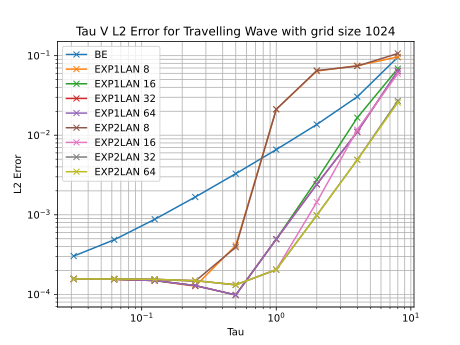
\includegraphics[width=1\textwidth]{Graphs/TravellingWave/Tau V L2 Error for Travelling Wave with grid size 1024.png} % Change filename to your image
        \caption{$\tau$ vs $L_2$ with grid size 1024}
        \label{fig:plot1}
    \end{minipage}\hfill
    \centering
    \begin{minipage}{0.49\textwidth}
        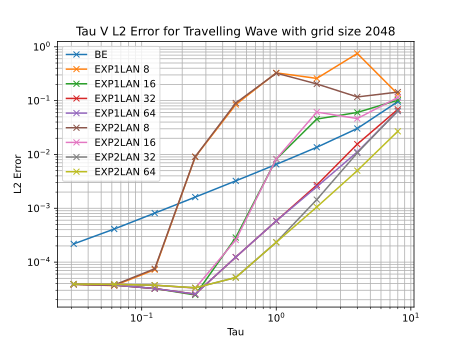
\includegraphics[width=1\textwidth]{Graphs/TravellingWave/Tau V L2 Error for Travelling Wave with grid size 2048.png} % Change filename to your image
        \caption{$\tau$ vs $L_2$ with grid size 2048}
        \label{fig:plot2}
    \end{minipage}\hfill
\end{figure}

First see that all of the methods tested converge, tending towards the discritisation error.
The discritisation error is smaller on the more detailed grid.
The Krylov methods converge faster than the backwards Euler method.
We notice that when a smaller Krylov subspace is used that the expoenntial methods only start to converge for a sufficiently small $\tau$.
Likewise when these methods start to converge we observe that they perform simillarly to the methods using a larger subspace, however they will require fewer operator calls.
This suggests that for sufficient small time steps a shallower subspace may suffice.
Likewise for the converse that larger timesteps require a deeper krylov subspace.

Now we compare the error with the number of calls to the operator.
These operator calls are needed for computing $N$ which is used with the matrix free methods as described above as well as for computing the non-linear term $R$.

\begin{figure}[H]
    \centering
    \begin{minipage}{0.49\textwidth}
        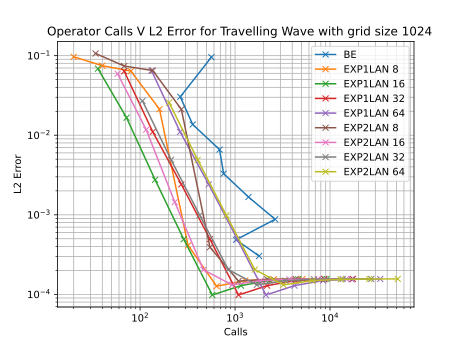
\includegraphics[width=1\textwidth]{Graphs/TravellingWave/Operator Calls V Error for Travelling Wave with grid size 1024.png} % Change filename to your image
        \caption{$\tau$ vs $L_2$ with grid size 1024}
        \label{fig:plot1}
    \end{minipage}\hfill
    \centering
    \begin{minipage}{0.49\textwidth}
        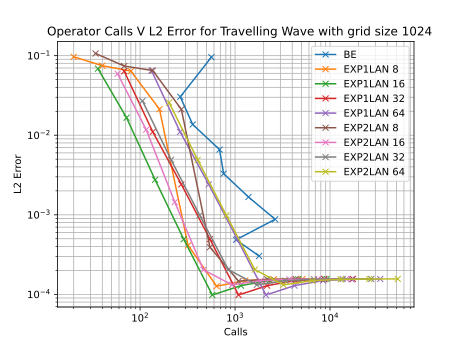
\includegraphics[width=1\textwidth]{Graphs/TravellingWave/Operator Calls V Error for Travelling Wave with grid size 1024.png} % Change filename to your image
        \caption{$\tau$ vs $L_2$ with grid size 2048}
        \label{fig:plot2}
    \end{minipage}\hfill
\end{figure}

We see that as expected that when a larger Krylov subspace is used that more calls to the operator are required.
We also observe that the exponential methods outperform the BE by achieving a lower error with fewer calls to the operator.

Here we present the experimental orders of convergence for the grid size 1024.

\begin{table}[H]
    \centering
    \begin{tabular}{| c | c | c | c}
    \hline
    BE & EXP1LAN 64 & EXP2LAN 64 \\
    \hline
    1.656175178817219 & 2.5200121901844423 & 2.427488988868435 \\
    1.159963039219372 & 2.147211103525317 & 2.2448741639287576 \\
    1.0543798412512431 & 2.1084233436748687 & 2.175268892119002 \\
    1.0188791686457326 & 2.235535140373336 & 2.176237872787299 \\
    1.0016513655730614 & 2.2847781778148475 & 0.6355415381730404 \\
    0.9874831778164389 & -0.3463812590562603 & -0.1610890501147955 \\
    0.9808216274859436 & -0.2097197508087928 & -0.0545528584432596 \\
    0.919336864575657 & -0.051644372942987 & -0.01407844052927163 \\
    \hline
    \end{tabular}
    \caption{Experimental orders of convergence}
    \label{tab:EOCs}
\end{table}


We observe that the rate of convergence for the second order method was inline with what has been shown analytic\cite{Huang2022} at a rate of $2$.
The first order method converges with a rate of 2 despite an expectation of a rate of $1$\cite{Huang2022}.
The exponential methods stop converging as they reach the discritisation error.
The backwards euler converges at the rate expceted of 1.

\subsection{A 2D Allen Cahn Problem}

We will now look into the two dimentional Allen Cahn Problem given by:
\begin{align*}
    u_t &= -\Delta u + u (u^2-1) \text{ } \Omega=[0,1]\times[0,1]
\end{align*}
With Neumann boundary conditions.
The initial condition is chosen by randomly setting points on the grid from a uniform distribution in the range $-0.9,0.9$.
The same randomly generated initial condition will be used for each test.
As we do not have an exact solution, we will use the backwards Euler method with a timestep of $\tau = 10^{-4}$ to genarate a referance solution.
We will compare the backwards Euler method to the first and second order expoenntial integrator methods described above.
The tests are run on a $60\times60$ grid with the end time being $t_e=24$.
The error is computed by calculating the $L_2$ error between the prediction of the chosen stepper and the reference solution. 
Below we present our results.

\subsubsection{Experimental Results}

We begin by compairing the timestep size $\tau$ to the $L_2$ error for the different methods.

\begin{figure}[H]
    \centering
    \begin{minipage}{0.49\textwidth}
        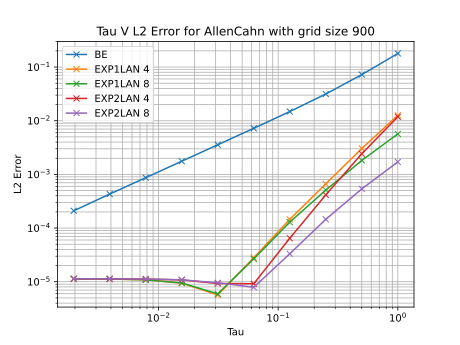
\includegraphics[width=1\textwidth]{Graphs/AllenCahn/Tau V L2 Error for AllenCahn with grid size 900.png} % Change filename to your image
        \caption{$\tau$ vs $L_2$ with grid size 900}
        \label{fig:ACtauE}
    \end{minipage}\hfill
    \centering
    \begin{minipage}{0.49\textwidth}
        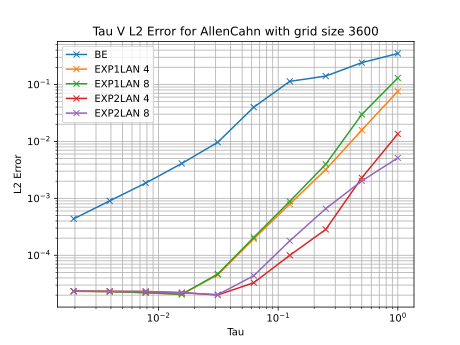
\includegraphics[width=1\textwidth]{Graphs/AllenCahn/Tau V L2 Error for AllenCahn with grid size 3600.png} % Change filename to your image
        \caption{$\tau$ vs $L_2$ with grid size 3600}
        \label{fig:ACtauE1024}
    \end{minipage}\hfill
\end{figure}

We observe convergence in both expoential methods for both krylov sizes.
These methods significantly outperform the backwards Euler method, simillar to the traveling wave Allen Cahn problem given above.
For this problem a relatively shallow subspace has been used compaired to above and appears to be sufficient.

Below as before we present the number of calls to the operator against the error.
\begin{figure}[H]
    \centering
    \begin{minipage}{0.49\textwidth}
        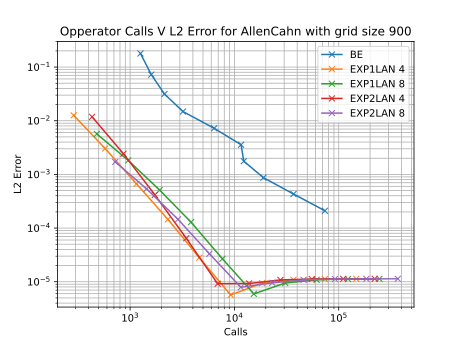
\includegraphics[width=1\textwidth]{Graphs/AllenCahn/Operator Calls V Error for AllenCahn with grid size 900.png} % Change filename to your image
        \caption{Operator calls vs $L_2$ with grid size 900}
        \label{fig:plot1}
    \end{minipage}\hfill
    \centering
    \begin{minipage}{0.49\textwidth}
        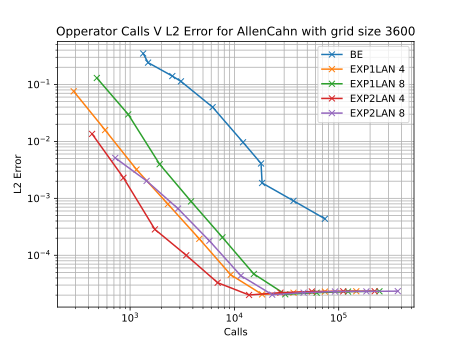
\includegraphics[width=1\textwidth]{Graphs/AllenCahn/Operator Calls V Error for AllenCahn with grid size 3600.png} % Change filename to your image
        \caption{Operator calls vs $L_2$ with grid size 3600}
        \label{fig:plot2}
    \end{minipage}\hfill
\end{figure}
For both methods we see that to achive a lower error requires more calls to the operator.
We see that in terms of performance the backwards Euler method performs significantly worse in comparison to both of the expoential methods.

Here we present the experimental orders of convergence on a grid size of 3600.

\begin{table}[H]
    \centering
    \begin{tabular}{| c | c | c |}
    \hline
    BE & EXP1LAN 8 & EXP2LAN 8 \\
    \hline
    0.5336772856567727 & 2.124425468811078    & 1.3416905476319223 \\
    0.7835756762460372 & 2.905742997002231    & 1.6172444544625373 \\
    0.3087677833100485 & 2.1667343028183392   & 1.8766417619133886 \\
    1.504631886802277  & 2.0994616006682154   & 2.034301870712038 \\
    2.0486348034911237 & 2.13577903687606     & 1.1061518243743675 \\
    1.237052619854426  & 1.184386408121027    & -0.11660694297267732 \\
    1.1376542802507796 & -0.09373274955254216 & -0.06785678855256895 \\
    1.0396362359013922 & -0.06516215516412459 & -0.005698148120031917 \\
    1.0482179972577244 & -0.01797864948877803 & -0.01442779444997218 \\
    \hline
    \end{tabular}
    \caption{Experimental orders of convergence}
    \label{tab:reduced_data}
\end{table}

Again we observe first order convergence for the backwards Euler methods and second order convergence for the two exponential integrator methods.

\subsection{Reaction Diffusion}

For both of the above problems the first order exponential method converged with rate 2.
In order to verify correct implementation, and to be able to compare the backwards Euler method to the first order expoenential method in a "fairer" way we study the following reaction diffusion problem\cite{Huang2022}.

\begin{align*}
    u_t &= -\frac12\Delta u + \frac12 \pi^2u + \frac12 \pi^2 e^{-\pi^2t}sin(\pi x)sin(\pi y) \text{ } (x,y)\in\Omega t\in\times[0,t_e]\\
    u(0,x,y) &= (sin(\pi x) - 1)sin(\pi y) \text{ } (x,y)\in \Omega
\end{align*}

With the following exact solution:

\begin{align*}
    u(t, x, y) &= e^{-\pi^2t}(sin(\pi x) - 1)sin(\pi y)
\end{align*}

With homogenous Dirichlet boundary conditions.
Where $\Omega = (\frac12, \frac52)\times(0,1)$ and our end time is given by $t_e = 0.1$.
We run our tests on grid sizes of $128\times64$ and $256\times128$ and use times steps sizes of $\tau=\frac{0.1}{2^i}$ for $i = 0,1,...,4$


We begin by compairing the timestep size $\tau$ to the $L_2$ error for the different methods.
\begin{figure}[H]
    \centering
    \begin{minipage}{0.49\textwidth}
        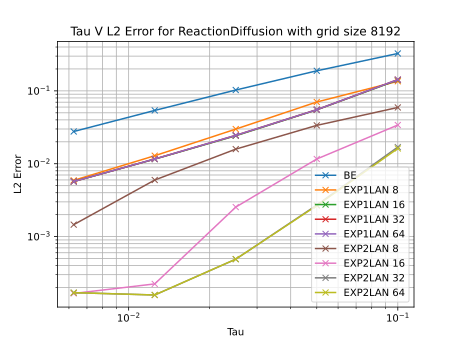
\includegraphics[width=1\textwidth]{Graphs/ReactionDiffusion/Tau V L2 Error for ReactionDiffusion with grid size 8192.png} % Change filename to your image
        \caption{$\tau$ vs $L_2$ with grid size 8192}
        \label{fig:ACtauE}
    \end{minipage}\hfill
    \centering
    \begin{minipage}{0.49\textwidth}
        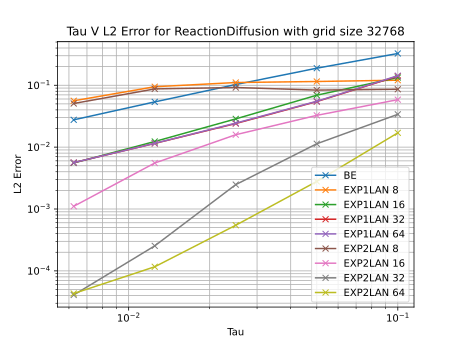
\includegraphics[width=1\textwidth]{Graphs/ReactionDiffusion/Tau V L2 Error for ReactionDiffusion with grid size 32768.png} % Change filename to your image
        \caption{$\tau$ vs $L_2$ with grid size 32768}
        \label{fig:ACtauE1024}
    \end{minipage}\hfill
\end{figure}
All methods appear to converge to the spacial discritisation error.
As above, we observe that the Krylov subspace must be sufficiently deep in order to be accurate.
In this example we can see that the second order method converges at a faster rate than the first order method as the slop for the second order method is steaper.
We also see that backwards Euler method has a higher error for a given value of $\tau$ for both methods.

Below as before we present the number of calls to the operator against the error.
\begin{figure}[H]
    \centering
    \begin{minipage}{0.49\textwidth}
        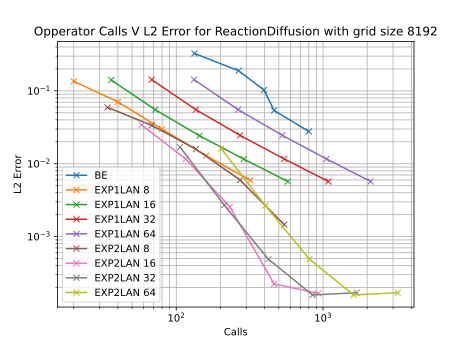
\includegraphics[width=1\textwidth]{Graphs/ReactionDiffusion/Operator Calls V Error for ReactionDiffusion with grid size 8192.png} % Change filename to your image
        \caption{Operator calls vs $L_2$ with grid size 1024}
        \label{fig:plot1}
    \end{minipage}\hfill
    \centering
    \begin{minipage}{0.49\textwidth}
        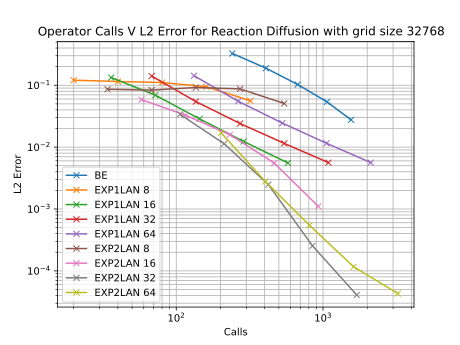
\includegraphics[width=1\textwidth]{Graphs/ReactionDiffusion/Operator Calls V Error for ReactionDiffusion with grid size 32768.png} % Change filename to your image
        \caption{Operator calls vs $L_2$ with grid size 2048}
        \label{fig:plot2}
    \end{minipage}\hfill
\end{figure}
Here we see that for all methods more operator calls are required to produce results with a smaller error.
The expoenential methods achieved a given error with fewer operator calls that the backwards Euler method.
The second order methods required fewer operator calls for a given error that the first order method, especially as the number of calls increased.


Here we present the experimental orders of convergence.
\begin{table}[H]
    \centering
    \begin{tabular}{| c | c | c |}
    \hline
    BE & EXP1LAN 64 & EXP2LAN 64 \\
    \hline
    0.7901637433430926 & 1.3717257454910614    & 2.608595189003896 \\
    0.8767440969959281 & 1.1734740319093697    & 2.3519399751018963 \\
    0.9320179419151513 & 1.0828183773958644   & 2.229913816965242\\
    0.963545660578168  & 1.03777329582159   & 1.4358363206568961 \\
    \hline
    \end{tabular}
    \caption{Experimental orders of convergence}
    \label{tab:reduced_data}
\end{table}

Now we observe the expected results, with the first order expoenential method converging at rate $1$ and the second order method converging at rate $2$.
\section {Snowflakes}
Here we begin to look in the phase boundary of the formation of a snowflake.
We will use an adaptive grid and compaire the first and second order exponential integrator methods.
We will also compare the limitations of these methods for differnt krylov sizes.
\subsection{Formulation of problem}

We condider the problem on a domain $\Omega = \mathbb{R}_+ \times [4, 8] \times [4, 8]$.
The equaitions govening this phase boundary problem are as follows.
\begin{align*}
    \tau \frac{\partial \phi}{\partial t} &= \nabla \cdot D\nabla\phi +  \phi(1-\phi)m(\phi,T)\\
    \frac{\partial T}{\partial t} &= D_T \nabla ^2T + \frac{\partial \phi}{\partial t}\\
    \intertext{Substituting in $\frac{\partial \phi}{\partial t}$ into the second equation and rewriting in weak form gives the following}
    \int \frac{\partial \phi}{\partial t} v_{\phi} &=  \frac 1{\tau}\int \phi(1-\phi)m(\phi,T)v_{\phi} - D \nabla \phi \cdot \nabla v_{\phi}\\
    \int \frac{\partial T}{\partial t} v_T &= \int \frac 1{\tau}(\phi(1-\phi)m(\phi,T)v_T - \nabla v_T \cdot D \nabla \phi) - D_T \nabla v_T \cdot \nabla T
\end{align*}
\begin{figure}[h]
    \centering
    \includegraphics[width=0.5\textwidth]{Snowflakes/EXP1LAN/Snowflake_2--problem_1.0_0_16.png} % Change filename to your image
    \caption{Initial condition}
    \label{fig:initial}
\end{figure}
With an initial condition of: \ref{fig:initial}
\begin{align*}
    \phi(0,x,y) &= \begin{cases} 
      1 & (x - 6)^2 + (y - 6)^2 \leq 0.3 \\
      0 & \text{otherwise} \end{cases}\\
    T(0,x,y) &= -0.5 (0,x,y)\in \Omega
\end{align*}

Where we have that

\begin{align*}
    m(\phi, T) &= \phi - \frac 12 - \frac{\kappa_1}{\pi}arctan(\kappa_2 T)\\
    D &= \alpha^2(1+c\beta)
    \begin{pmatrix}
        1+c\beta & -c\frac{\partial\beta}{\partial\psi}\\
        c\frac{\partial\beta}{\partial\psi} & 1+c\beta
    \end{pmatrix}\\
    \text{With }\beta &= \frac{1-\Phi^2}{1+\Phi^2}\\
    \Phi &= tan(\frac N2\psi)\\
    \psi &= \theta + arctan(\frac{\frac{\partial \phi}{\partial y}}{\frac{\partial \phi}{\partial x}})\\
\end{align*}
and with the following constants
\begin{align*}
    \begin{matrix}
    D_T = 2.25 & \alpha = 0.015 & \tau = 3\cdot 10^{-4} & \kappa_1 &= 0.9\\
    \kappa_2 = 20 & c = 0.02 & N = 6 & \theta = \frac{\pi}8
    \end{matrix}
\end{align*}

\subsection{Numerical Solutions}
Here we begin the comparison of the differnet methods.
For all of them we will use a time step size of $0.0005$ and will run untill and end time of $0.1$.\\

We begin looking at the results for the first order method with a krylov subspace of dimention $16, 32$.

\begin{figure}[H]
    \centering
    \begin{minipage}{0.49\textwidth}
        \includegraphics[width=1\textwidth]{Snowflakes/EXP1LAN/Snowflake_2--problem_1.0_10_16.png} % Change filename to your image
        \caption{from First order exponential integrator with krylov size $16$}
        \label{fig:first order 16}
    \end{minipage}\hfill
    \centering
    \begin{minipage}{0.49\textwidth}
        \includegraphics[width=1\textwidth]{Snowflakes/EXP1LAN/Snowflake_2--problem_1.0_10_32.png} % Change filename to your image
        \caption{from First order exponential integrator with krylov size $32$}
        \label{fig:first order 32}
    \end{minipage}\hfill
\end{figure}

We observe that the snowflakes generated by both krylov sizes are near identical, 
suggesting that setting the dimention of the krylov space to $16$ is sufficient for this problem.\\

Moving on to the second order method we use a krylov size of $, $.

\subsection{Limitations}
Now we compare the limitations of the first and second order exponential methods when the dimention of the krylov space is smaller that for what we saw above.
We compare it for krylov sizes of $8$ and $12$.

When an exponentially small subspace is used such as $8$ as shown in figure %cite figure
we observe that the snowflake continuses to grow in the shape of a smooth hexagon without forming any dendrites.
When we use a subspace of size $12$ we observe that while dendrites now form they are stubbier and produce less branching.
%\section{Parallelization}

Here we investigate how well the model can be parallelized.
We will investigate this for both the travelling wave problem as well as for modeling 2D snowflake growth.
For both, we will investigate how these mehtods scale on different numbers of cores for differnet krylov subspaces and measure timings accordingly.
These methods will be compared to the backwards euler method.

\subsection{Travelling Wave Allen Cahn}

We will compare the first and second order methods for a variety of gridsizes and krylov subspace sizes.
The grid sizes to be used are as follows: to be decided and the krylov sizes will be: to be decided.


\subsection{2D Snowflake Modeling}

Here we look at how well the krylov methods scale in relation to krylov subsapce size using subspaces of dimension ~.
The grid complexity is govened by adaptive mesh refinement.

\begin{table}[H]
    \centering
    \begin{tabular}{| c | c c | c c | c c | c c | c c | c c |}
    \hline
    Cores & \multicolumn{2}{c|}{BE} & \multicolumn{2}{c|}{EXP1LAN 16} & \multicolumn{2}{c|}{EXP1LAN 32} & \multicolumn{2}{c|}{EXP2LAN 16} & \multicolumn{2}{c|}{EXP2LAN 32} \\
    \hline
    & T & CR & T & CR & T & CR \\
    \hline
    1  & 0 & 0 & 0 & 0 & 0 & 0 \\
    2  & 0 & 0 & 0 & 0 & 0 & 0 \\
    4  & 0 & 0 & 0 & 0 & 0 & 0 \\
    8  & 0 & 0 & 0 & 0 & 0 & 0 \\
    16 & 0 & 0 & 0 & 0 & 0 & 0 \\
    \hline
    \end{tabular}
    \caption{Reduced Data Table}
    \label{tab:reduced_data}
\end{table}

\section{Double Slit Wave Model}

In this section, we look into applying these exponential steppers to the computation of solutions to the wave eqaution.
We will look into solutions the the double slit wave problem:

\subsection{Formulation of the Problem}
Where our domain is given by $\Omega$, we write the problem as:
\begin{align*}
    \psi_{tt}\psi &= \nabla \psi \quad x \in \Omega, 0<t\leq T\\
    \psi &= \frac{1}{10\pi} sin(10\pi t) x \in S_L
\end{align*}
where $T=3$ is our end time for the simulation and $S_L$ denotes the left side of the domain $\Omega$ this will be the source of our waves.
We can use $\psi_t = -p$ to get the following:
\begin{align*}
    \psi_t &= -p\\
    p_t &= \nabla \psi\\
    \psi &= \frac{1}{10\pi} sin(10\pi t) x \in S_L
\end{align*}
This equation is now compatable with the time steppers that we are using.

\subsection{Numerical Solutions}
We can now compare backwards euler and the two exponential integrator methods.
First we show the the domain as well as a solution computed with the backwards Euler method.
For the backwards Euler a time step of $\tau = 0.001$ was found to be optimal, with larger timesteps causing numerical issues and smaller timesteps requiring excessive computation.

\begin{figure}[H]
    \centering
    \begin{minipage}{0.49\textwidth}
        \includegraphics[width=1\textwidth]{Wave/DoubleSlit_0_1.0_0_64.png} % Change filename to your image
        \caption{Domain $\Omega$ with grid displayed}
        \label{fig:second order 16}
    \end{minipage}\hfill
    \centering
    \begin{minipage}{0.49\textwidth}
        \includegraphics[width=1\textwidth]{Wave/BE/DoubleSlit_0_0.1_10_64.png} % Change filename to your image
        \caption{Solution at time $T=3$ computed using the backwards euler method}
        \label{fig:second order 32}
    \end{minipage}\hfill
\end{figure}

We now compare this to the first and second order exponential integrator methods.
Note that due the fact that the linear term given by $DN(u)$ is not symetric we cannot use the Lancoz method for computing our matrix exponential.
As a result the Arnoldi alorithm for the matrix exponential has been used here exculively.
\begin{figure}[H]
    \centering
    \begin{minipage}{0.49\textwidth}
        \includegraphics[width=1\textwidth]{Wave/EXP1ARN/DoubleSlit_0_2.0_10_24.png} % Change filename to your image
        \caption{Solution at time $T=3$ computed Using the first order exponential integrator with timestep $\tau = 0.02$ and a Krylov size of $24$}
        \label{fig:second order 16}
    \end{minipage}\hfill
    \centering
    \begin{minipage}{0.49\textwidth}
        \includegraphics[width=1\textwidth]{Wave/EXP2ARN/DoubleSlit_0_2.0_10_24.png} % Change filename to your image
        \caption{Solution at time $T=3$ cmoputed using the second order exponential integrator with timestep $\tau = 0.02$ and a Krylov size of $24$}
        \label{fig:second order 32}
    \end{minipage}\hfill
\end{figure}

We see that the first and second order exponential methods using the Arnoldi algorithm are capable of producing results equivalent to that of the backwards Euler method.

\subsection{Performance}
We now observe the performance differences between the methods.
For this, the number of calls to the operator is again used in order to measure performance.
We present the methods used and the operator calls in the table below:

\begin{table}[H]
    \centering
    \begin{tabular}{| c | c | c | c |}
    \hline
    Method & Required $\tau$ & Krylov size & Operator Calls\\
    \hline
    Backwards Euler & 0.001 & - & 119362 \\
    First Order Expoenntial & 0.02 & 24 & 7800 \\
    Second Order Expoenntial & 0.02 & 24 & 12300 \\
    \hline
    \end{tabular}
    \caption{Performance of Various Methods}
    \label{tab:reduced_data}
\end{table}

We observe that Backwards Euler method requires significantly more calls to the operator that both the first and second order exponential methods.
The second order method requires more calls to the operator than the first order method.
This suggest that these methods may be effective for computing solutions to the wave equation.
\section{Rising Bubble}

Here we will look into computing a rising bubble, in order to investigate how well these methods work for problems in the modeling of atmospheric processes.
\subsection{Formulation of Problem}
The problem is given by the following equations\cite{Bryan2002}:
\begin{align*}
    \frac{\partial u_i}{\partial t} &= -\frac{\partial u_i u_j}{\partial x_j} + u_i\frac{\partial u_j}{\partial x_j} - c_p \theta \frac{\partial \pi}{\partial x_i} \\
    \frac{\partial \pi}{\partial t} &= -\frac{\partial u_j \pi}{\partial x_j} + \pi\frac{\partial u_j}{\partial x_j} - \pi \frac{R}{c_v}\frac{\partial u_j}{\partial x_j} \\
    \frac{\partial \theta}{\partial t} &= -\frac{\partial u_j \theta}{\partial x_j} + \theta\frac{\partial u_j}{\partial x_j}
\end{align*}
where Einstein's summing notation is used.
We use a domain $\Omega = (0,1000) \times (0,2000)$.
The constants are given by:
\begin{align*}
    \begin{matrix}
    c_p = 1005 & c_v = 717.95 \\
    R = c_p - c_v 
    \end{matrix}
\end{align*}

We enforce reflective boundary conditions along the sides of the domain.
The initial condtions are as follows:
\begin{align*}
    u_i &= 0\\
    \pi(0,x,y) &= \pi_0\\
    \theta &= 0
\end{align*}
where $\pi_0$ is shown below
\begin{figure}[H]
    \centering
    \begin{minipage}{1\textwidth}
        \includegraphics[width=1\textwidth]{Bubble/initial.png} % Change filename to your image
        \caption{Initial Condition of $\pi_0$}
        \label{fig:first order 8 0.5}
    \end{minipage}
\end{figure}
\subsection{Numerical Solutions}
We run our simulations on a finite volume mesh.
The grid is rectangular and of dimension $64\times 128$.
We use a timestep of $\tau = 1.8$ as this was optimal when used with the backwards Euler method.
We plot the value of $\pi$ at time $t=4000$.
\begin{figure}[H]
    \centering
    \begin{minipage}{0.49\textwidth}
        \includegraphics[width=1\textwidth]{Bubble/EXP1ARN32.png} % Change filename to your image
        \caption{from first order exponential integrator with Krylov size $32$}
        \label{fig:first order 8 0.5}
    \end{minipage}\hfill
    \centering
    \begin{minipage}{0.49\textwidth}
        \includegraphics[width=1\textwidth]{Bubble/EXP1ARN64.png} % Change filename to your image
        \caption{from first order exponential integrator with Krylov size $64$}
        \label{fig:first order 10 0.5}
    \end{minipage}\hfill
\end{figure}
\begin{figure}[H]
    \centering
    \begin{minipage}{0.49\textwidth}
        \includegraphics[width=1\textwidth]{Bubble/EXP2ARN32.png} % Change filename to your image
        \caption{from second order exponential integrator with Krylov size $32$}
        \label{fig:first order 8 0.5}
    \end{minipage}\hfill
    \centering
    \begin{minipage}{0.49\textwidth}
        \includegraphics[width=1\textwidth]{Bubble/EXP2ARN64.png} % Change filename to your image
        \caption{from second order exponential integrator with Krylov size $64$}
        \label{fig:first order 10 0.5}
    \end{minipage}\hfill
\end{figure}
For Krylov sizes above $64$ the computed solution didn't change.
The solution computed with a Krylov size of $64$ was the same as the solution by the backwards Euler method as well as for smaller $\tau$.
We therefore conclude that this is close to the true solution.

\subsection{Performance}
We now observe the performance differences between backwards Euler and the exponential integrators.
The number of calls to the operator is again used in order to measure performance.
We present the methods used and the operator calls in the table below:

\begin{table}[H]
    \centering
    \begin{tabular}{| c | c | c | c |}
    \hline
    Method & Krylov size & Operator Calls\\
    \hline
    Backwards Euler & - & 156879 \\
    First Order Exponential & 32 & 151640 \\
    First Order Exponential & 64 & 303280 \\
    Second Order Exponential & 32 & 227460 \\
    Second Order Exponential & 64 & 454920 \\
    \hline
    \end{tabular}
    \caption{Performance of Various Methods}
    \label{tab:reduced_data}
\end{table}

We see that these exponential integrator methods required more operator calls than the backwards Euler method to achieve comparable results for this timestep size.


Further studies of these methods could include finding the optimal tau for these methods that minimises the number of operator calls.
It would also make sense to explore the possible values of $m$ in between 32 and 64 as we would expect to find that these methods converge to the expceted solution for a Krylov size between these two values.
However, due to time constraints on the project, it has not been possible to gather this information.


\section{3D Crystal}
We now begin looking into the modeling of a 3D Crystal.
\subsection{Formulation of Problem}
We employ the phase field model as described by \cite{Bollada2023}.
\begin{align*}
    \dot \phi &= \nabla \cdot \frac{\partial}{\partial \nabla \phi}(\frac12 A^2)-\frac{Omega'(\phi)}{\delta^2} - \frac{g'(\phi)(\mu_0-\mu)\Delta c}{\lambda \delta^2}\\
    \dot \mu &= a\nabla \cdot D \nabla \mu - a \Delta c g'(\phi)\dot \phi\\
    \phi(0,x) &= \phi_{t=0}\\
    \mu(0,x) &= \mu_{t=0}
\end{align*}
For some initial conditions $\phi_{t=0}$ and $\mu_{t=0}$ and with an anisotropy given by $A$.
\begin{align*}
    \phi_{t=0} &= \frac{1}{1+e^{\frac{-\sqrt{x^2 + y^2 + z^2}-R_0}{\delta}}}\\
    \mu_{t=0} &= \phi_{t=0} - \phi_{t=0}a(\bar c - c_s)
\end{align*}
The constants are given by:
\begin{align*}
    \begin{matrix}
    c_L = 0.9 & c_S = 0.5 & \mu_0 = 1 & \mu_{\inf} = 0.04 & a = 4 & D_L= \frac{1}{12} & D_S = 10^{-4}D_L\\
    \Delta c = c_L - c_S & \lambda = \frac{3R_c\Delta c^2}{\delta} & R_c = 10 & R_0 = 20 & \delta = 2 & \epsilon = 0.02\\
    \end{matrix}
\end{align*}

We will observe two different anisotropies.
The first a "cubic" anisotropy given by:
\begin{align*}
    A &= \sum_i \sqrt{\frac{\partial \phi}{\partial x^i}^2 + \epsilon^2(\frac{\partial \phi}{\partial x^1}^2 + \frac{\partial \phi}{\partial x^2}^2 + \frac{\partial \phi}{\partial x^3}^2)}
\end{align*}
and an octohedral anisotropy given by \cite{Bollada2015}:
\begin{align*}
    A &= A_0 (1 + \bar \epsilon(n^4_x+n^4_y+n^4_z))
\end{align*}
where we have that $A_0 =1 -3\epsilon$ and $\bar \epsilon = \frac{4\epsilon}{1-3\epsilon}$.


\subsection{Numerical Solutions}

\section{Conclusion}

This project has investigated the use of Krylov subspace methods, specifically Arnoldi and Lanczos alongside exponential integrators to provide numerical solutions to PDEs.
We have been able to demonstrate that this combination of methods can provide accurate solutions to PDEs with reduced computational cost relative to the backwards Euler method.
We have also begun to develop some error analysis of these methods in order to gain insight into how these Krylov methods affect the rate of convergence.
These methods show much promise for parabolic PDEs, especially phase boundary problems such as crystal growth.

Throughout this project, the size of the Krylov subspace played an important role in determining the accuracy of these results as well as performance demands.
Deeper Krylov subspaces yielded lower error, but had the downside of incurring a greater computational cost.
Further research could focus on how adapting the depth of this Krylov subspace dynamically during run time could improve performance such as with the KIOPS\cite{Gaudreault2018} method.

While much of our work focused on parabolic PDEs, we also showed that these methods may have possible application beyond the scope of parabolic PDEs.
These methods appeared effective for modeling the wave equation as well as showing potential in the modeling of atmospheric processes.
Further work could focus on applying these methods to a wider range of problems in order to properly understand the extent of their application, as well as how these methods apply to other spacial discretizations such as finite volume and finite difference.


\pagebreak

{\Huge \bf Bibliography}

\bibliographystyle{plain}
\bibliography{References.bib}
\bigskip

% These are examples of the book titles as they can be put in. 
% You can use different labeling methods, if you prefer, 
% e.g., just enumerating the items  as [1], [2], etc.,
% instead of making them [ATLAS], [B], etc.
% Or use bibtex



\end{document}
